
\lhead[{\bfseries \thepage}]{ \rightmark}
\rhead[Resum de la tesi \leftmark]{\bfseries \thepage}

%\markboth{Resumen de la tesis}{Resumen de la tesis}
%\addcontentsline{toc}{part}{Resumen de la tesis} 
\label{partIII}

%\begin{comment}
 \newcounter{alphasect}

 \renewcommand\thesection{%
 \ifnum\value{alphasect}=1%
A%%
 \else
\ifnum\value{alphasect}=2%
B%%
\else
\ifnum\value{alphasect}=3%
C%%
\else
\ifnum\value{alphasect}=4%
D%%
\else
 \arabic{section}%%
 \fi\fi\fi\fi}%

 \newenvironment{asection}{%
 \setcounter{alphasect}{1}%%
 }{%
 \setcounter{alphasect}{0}%%
 }%

 \newenvironment{bsection}{%
 \setcounter{alphasect}{2}%%
 }{%
 \setcounter{alphasect}{0}%%
 }%
%\end{comment}


\setcounter{section}{0}

\chapter*{Recerca de la producció associada de bosó de Higgs i un quark top amb dos leptons i tau hadrònic a l'estat final}
\addcontentsline{toc}{chapter}{Resum de la tesi} 
\label{chap:resumen_val}

El Model Estàndard (SM) de la física de partícules és una teoria notablement exitosa, 
però també revela limitacions significatives. Aquest model unifica totes les partícules 
elementals que constitueixen l'univers conegut en una teoria única. Dins d'aquest marc, 
el quark $\text{top}$ i el bosó de Higgs desperten un interés especial, ja que poden 
contribuir a respondre algunes de les qüestions encara pendents. Aquesta tesi es 
centra en l'estudi d'aquestes dues partícules singulars i la seua interacció. El
marc teòric per a l'estudi de la física d'aquestes partícules es presenta 
la Secció \ref{chap:resumen_val:Teoria}.

Per dur a terme aquest estudi, s'han utilitzat dades de col·lisions protó-protó amb una 
lluminositat integrada de $140,\text{fb}^{-1}$, a una energia de centre de masses de 
$13,\text{TeV}$, recopilades pel detector ATLAS durant el Run 2 del Gran Col·lisionador 
d'Hadrons (LHC) l'Organització Europea per a la Recerca Nuclear (CERN). L'ATLAS 
és un el detector més gran de l'LHC, que és el més potent accelerador de partícules del 
món. El marc experimental en què s'emmarca aquest treball es descriu a la sección 
\ref{chap:resumen_val:Exp}. La recopilació de les dades, la generació de simulacions 
de Monte Carlo, i a reconstrucció i identificació dels objectes físics són descrits a
la Secció \ref{chap:ObjectReconstuction}

El decobriment del bosó de Higgs pels experiments ATLAS \cite{20121_ATLAS_HiggsDiscovery} 
i CMS \cite{201230_CMS_HiggsDiscovery} en 2012 va obrir un nou camp d'exploració en la física 
de partícules. Per comprendre millor el SM, és d'un gran interés determinar l'acoplament de Yukawa 
del bosó de Higgs amb el quark $\text{top}$ (\yt). Aquest quark és la partícula fonamental més massiva 
i, per tant, presenta l'acoplament més fort amb el bosó de Higgs.

La mesura directa de \yt només és possible al LHC a través de dues produccions associades 
del bosó de Higgs: amb un parell de quark-antiquark de $\text{top}$ (\ttH) i amb un quark $\text{top}$ 
solitari juntament amb un partó addicional (\tHq). Mentre que el \ttH permet només determinar la 
magnitud de \yt, l'única manera de mesurar simultàniament el seu signe i magnitud és mitjançant la
 producció \tH \cite{Demartin:2015uha}. L'observació d'un excés d'esdeveniments de senyal en 
 comparació amb la predicció del SM podria ser una evidència de nova física en termes de violació 
 de \CP a l'acoplament \yt.
 
 En aquest treball, es presenta una cerca de la producció \tHq a l'estat final definit 
per dos leptons lleugers carregats (electrons o muons) i un $\Ptau$ que es desintegra 
manera hadrònica. Aquesta configuració es coneix com a canal \dileptau.
Aquesta cerca presenta un repte a causa de l'extremadament petita secció eficaç del procés \tHq en general,
i sobretot pel canal final \dileptau, que representa només el 3.5\% de la producció total de \tHq.

Per distingir els esdeveniments de senyal \tHq dels de fons, s'han utilitzat tècniques d'aprenentatge automàtic. 
En concret, s'han utilitzat arbres de decisió potenciats (BDT) per definir regions enriquides de senyal, així com regions 
de control que limiten els processos de fons més importants. Els fons rellevants inclouen la producció de parells 
de quark-antiquark de $\text{top}$ sense i amb un bosó addicional (\ttbar, $t\bar{t}H$, $t\bar{t}W$ i $t\bar{t}Z$) i 
el bosó $Z$ juntament amb jets.


A més, per ajudar a identificar els esdeveniments de senyal dins les dades, la reconstrucció de l'esdeveniment juga 
un paper crucial. En situacions en què els leptons lleugers tenen la mateixa càrrega elèctrica, no és possible 
determinar a priori quin leptó prové del bosó de Higgs i quin prové del quark $\text{top}$. En aquest context s'ha 
desenvolupat una eina basada en un BDT per assignar exitosament l'origen. 

S'aconsegueix una supressió significativa dels esdeveniments de fons, imposant requisits estrictes d'identificació i aïllament 
per als electrons i muons. Al mateix temps, es demana als taus hadrònics que superin un discriminador basat en xarxes 
neuronals recurrents per reduir les identificacions errònies provinents dels jets.

Totes les ferramentes mencionades per a la recerca de processos \tH i el procediment per a l'anàlisi estan descrits a la 
Secció \ref{chap:resumen_val:tHq}.

%%%%%%%
%   Teoria   %
%%%%%%%
\section{Marc teòric}
\label{chap:resumen_val:Teoria}

\subsection{El Model Estàndard}
%https://www.quantamagazine.org/a-new-map-of-the-standard-model-of-particle-physics-20201022/
El Model Estàndard de Física de Partícules (SM) és un marc teòric que descriu els constituents 
bàsics de la matèria i les seues interaccions. És el model més àmpliament acceptat i confirmat experimentalment 
en la física de partícules.

El SM inclou dos tipus de partícules elementals, els fermions i bosons.
Els fermions són partícules subatòmiques que segueixen les regles de l'estadística de Fermi-Dirac. 
Aquest tipus de partícula es caracteritza per tenir un espín semienter i seguir el principi d'exclusió 
de Pauli, el qual estableix que dos fermions no poden ocupar el mateix estat quàntic simultaneament. 
Els fermions es divideixen en quarks i leptons. Ambdós tipus de fermions són els constituents bàsics 
de la matèria, però són diferents entre si.

D'una banda, els quarks són partícules que tenen càrrega elèctrica fraccionària. Els quarks són la unitat fonamental 
dels protons i els neutrons. Aquestes partícules es combinen en grups per formar hadrons (mesons i barions). Els barions 
inclouen els protons i els neutrons, que són les partícules subatòmiques més abundants en la matèria. Els mesons tenen un 
nombre parell de quarks, la qual cosa fa que tinguen espín enter i siguen bosons. Els quarks es divideixen en sis "sabors" 
diferents: amunt, avall, encant, estrany, superior i inferior. La forma més habitual de referir-se a ells és pel seu nom en anglés: 
up, down, charm, strange, top i bottom.

Els altres elements que componen el SM són els bosons, partícules amb espín enter que medien les 
interaccions fonamentals de la física. Els bosons de calibre (espín 1) són els responsables de descriure 
tres de les quatre forces fonamentals de la naturalesa\footnote{La gravetat queda fora del SM.}:

\begin{itemize}
	\item Interacció electromagnètica: Mediada pel fotó (\Pgamma), és la teoria que estudia 
	els fenòmens elèctrics i magnètics. Totes les partícules carregades interactuen entre si a 
	través d'aquesta força. Les principals característiques de la interacció electromagnètica són 
	el seu abast infinit i l'absència de massa dels seus portadors. És responsable de l'estabilitat 
	dels àtoms, ja que manté units els electrons en òrbita al voltant del nucli, i de la transmissió 
	de la llum i altres formes de radiació electromagnètica. La teoria que descriu aquesta interacció 
	es denomina electrodinàmica quàntica.
	
	\item Interacció nuclear feble: Mediat per dos bosons \PW (\PWplus i \PWminus) i el bosó \PZ. 
	Aquesta és responsable de la radioactivitat beta, en la qual un neutró es descompon en un 
	protó, un electró i un antineutrí. També és la força que mesura la desintegració del quark top 
	en un quark \Pbottom i un bosó \PW. A més, la interacció nuclear feble és crucial en el procés 
	de fusió en les estrelles, on es combinen protons per formar elements més pesants. Les forces 
	nuclear feble i electromagnètica es descriuen simultàniament per la teoria electrofeble.
	
	\item Interacció nuclear forta: Mediat pel gluó, és responsable de mantenir units els protons i 
	neutrons al nucli atòmic. És la interacció més forta de la naturalesa, però el seu abast d'acció 
	està limitat a distàncies subatòmiques. A causa del confinament per color de la teoria nuclear 
	forta, ni els glúons ni els quarks apareixen aïllats (excepte a altes energies). La teoria que descriu 
	aquesta interacció es diu cromodinàmica quàntica. Aquesta teoria, igual que l'electrodinàmica 
	quàntica i la teoria electrofeble, està basada en el formalisme de la teoria quàntica de camps.
\end{itemize}

La Figura \ref{fig:resumen_val:Teoria:SM} recull totes les partícules fonamentals descrites pel SM.

\begin{figure}
 	 \centering
 	  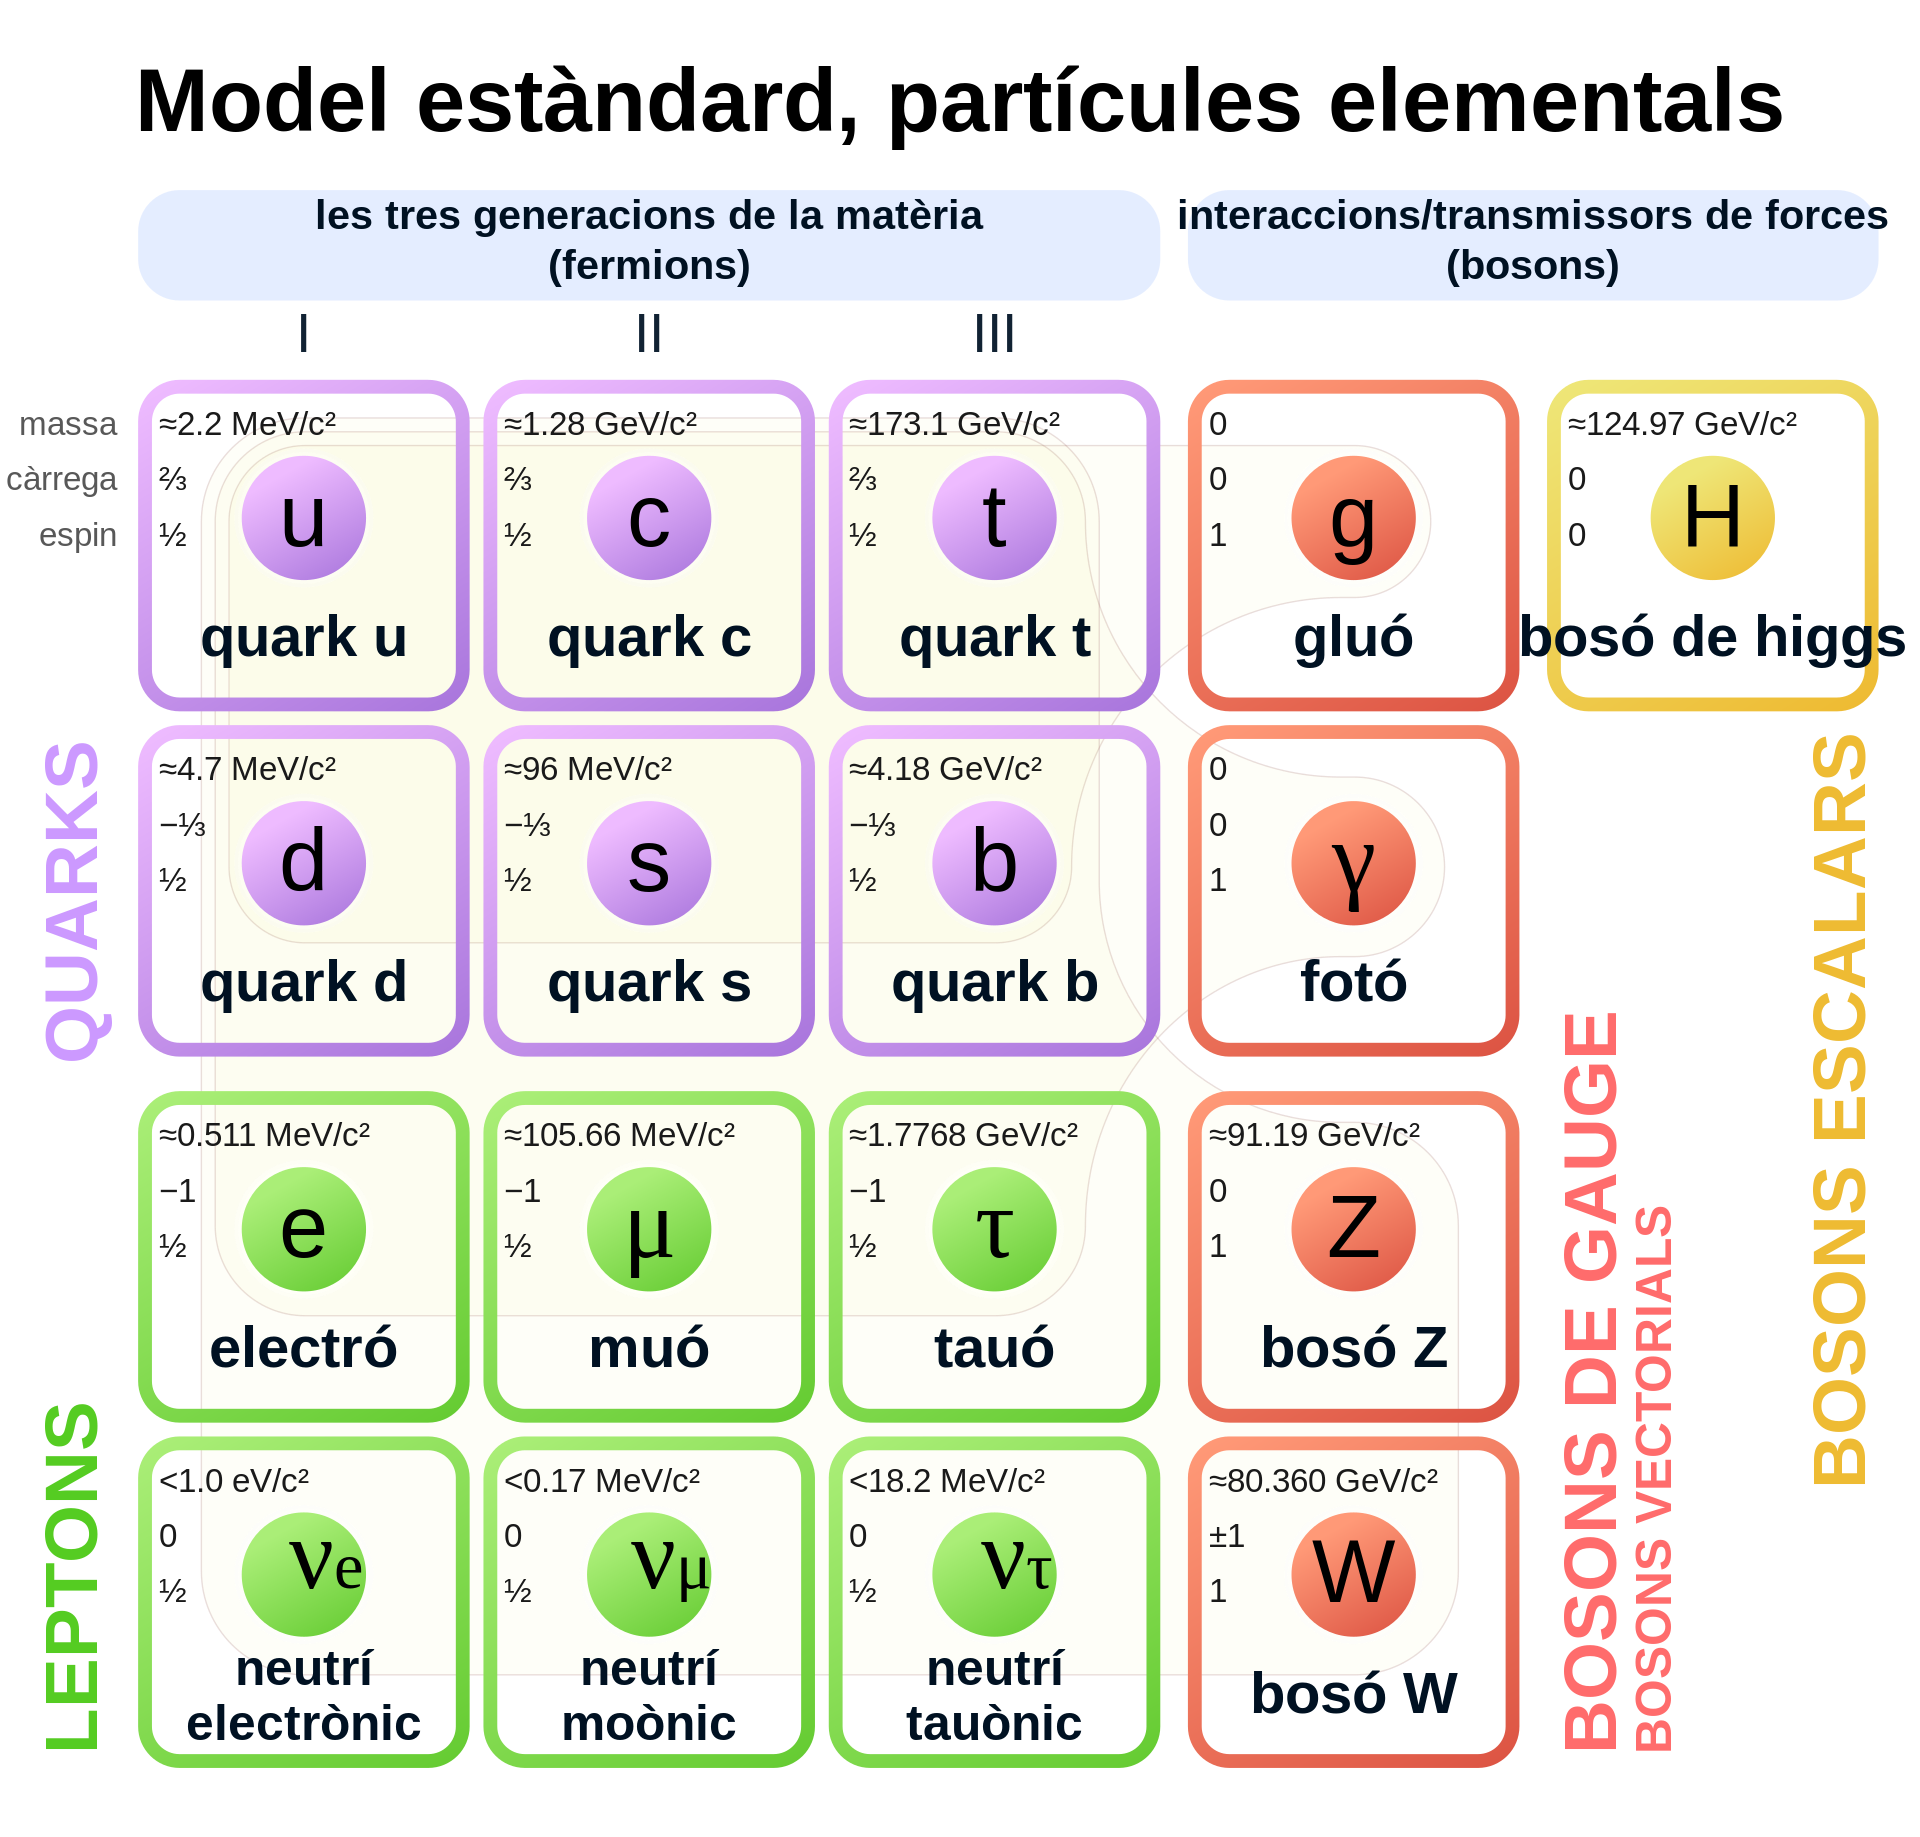
\includegraphics[width = 0.7\textwidth]{Chapter1/ZZ_Valencia_SM}
	  \caption{Model estàndard de les partícules elementals, amb les tres generacions de partícules de 
	  matèria, els bosons de gauge i el bosó de Higgs. Brown loops indicate which bosons (red) couple 
	  to which fermions (purple and green). Please note that the masses of certain particles are subject 
	  to periodic reevaluation by the scientific community.} 
	\label{fig:resumen_val:Teoria:SM}
\end{figure}


\subsection{La física del quark top}
\subsection{La física del bosó de Higgs}

%%%%%%%%%%
%   Experimento  %
%%%%%%%%%%
\section{L'experiment ATLAS del LHC al CERN}
\label{chap:resumen_val:Exp}
El Gran Col·lisionador d'Hadrons (LHC, per les seues sigles en anglés) és un accelerador de partícules que es troba 
al CERN (Centre Europeu per a la Recerca Nuclear o Laboratori Europeu de Física de Partícules Elementals), a 
Ginebra, Suïssa. Va ser dissenyat per a col·lisionar protons i ions pesats amb alta energia, el que permet als científics 
estudiar l'estructura subatòmica de la matèria i buscar noves partícules.

El LHC és una màquina d'avantguarda que utilitza tecnologia avançada per accelerar partícules fins a velocitats 
properes a les de la llum abans de xocar-les entre si. El funcionament 
del LHC es basa en l'ús de camps magnètics i radiofreqüències per accelerar les partícules carregades.
A continuació, els feixos de partícules són dirigits a col·lissionar en punts específics on es troben els detectors 
com ATLAS i CMS.
Aquestes col·lisions generen partícules secundàries que es 
detecten mitjançant una xarxa de detectors situats en el seu interior. Les dades recopilades d'aquestes col·lisions 
es fan servir per a investigar la física de partícules. Amb energies de $\CM = 13,$TeV, el LHC és l'accelerador de 
partícules més gran construït, la qual cosa constitueix una eina clau per a l'avanç de la ciència. 
Els quatre principals detectors que envolten el LHC són: ATLAS, CMS, LHCb i ALICE. 
El primer d'aquests és l'experiment en el qual es desenvolupa el treball que es descriu 
a aquesta tesi doctoral. 




%\subsection{El gran col·lisionador d'hadrons}
%\label{chap:resumen_val:Exp:LHC}
% Take inspiration from https://www.benasque.org/2022imfp/talks_contr/084_IMFP2022_ARuiz.pdf
%El funcionament del LHC es basa en l'ús de camps magnètics i radiofreqüències per accelerar les partícules carregades. Les partícules, ja siguin protons o ions pesats, són injectades en anells d'acceleració que estan interconnectats per tubs a alta pressió anomenats feixos. Aquests feixos de partícules són accelerats fins a prop de la velocitat de la llum mitjançant camps magnètics generats per superconductors. A continuació, els feixos de partícules són dirigits a col·lidir en punts específics on es troben els detectors com ATLAS i CMS.

%%%%%%%
%   ATLAS  %
%%%%%%%
\subsection{El detector ATLAS}
\label{chap:resumen_val:Exp:ATLAS}
El detector ATLAS s'utilitza per mesurar les propietats de les partícules resultants de les col·lisions d'hadrons. 
ATLAS té una estructura cilíndrica i és un dels detectors de partícules més grans del món, amb aproximadament 
46 metres de llargària i 25 metres de diàmetre. Està compost per diversos components i subcomponents. 
Cada un d'aquests sistemes s'encarrega de registrar un tipus d'informació diferent. En ordre de dins cap a fora, 
ATLAS està format per:
\begin{itemize}
\item Detector intern (ID): Aquest component és el més proper al punt de col·lisió i té com a finalitat 
	rastrejar les trajectòries de les partícules carregades. L'ID està format per tres subcomponents:
	\begin{itemize}
	\item Detector de Píxels: És la part més interna de l'ID. El material de detecció és silici de $250\,\mu$m 
		de grossor. Cada mòdul conté 16 xips de lectura i altres components electrònics. La unitat més petita 
		de detecció és el píxel ($50\times400 \,\mu$m), dels quals hi ha aproximadament 47000 per mòdul.
		La mida minúscula dels píxels està dissenyada per a un rastreig extremadament precís a prop del 
		punt d'interacció. Està compost per quatre capes dobles de tires de silici i té 6'3 milions de canals de 
		lectura i una àrea total de $61\,m^{2}$.
		
	\item Rastrejador de Semiconductors (SCT):  Té un concepte i una funció similars al Detector de Píxels, 
		però amb tires llargues i estretes en lloc de petits píxels, cosa que fa possible cobrir una àrea més gran.
		Cada tira té una mida de $80\,\mu$m per $12\,$cm. El SCT és la part més crítica del detector intern per al 
		rastreig bàsic en el pla perpendicular al feix, ja que mesura partícules en una àrea molt més gran que el 
		Detector de Píxels.
		
	\item El Rastrejador de Radiació de Transició (TRT): Del l'anglés Transition Radiation Tracker, és un 
		rastrejador de tubs de deriva\footnote{Straw chamber en anglés, es tracta d'un tub llarg amb un fil al centre i un
		gas que s'ionitza quan una partícula el travessa.}. Cada tub te un diàmetre 
		de $4\,$mm, una longitud de fins a $144\,$cm i està ple d'una mescla de gasos.
\end{itemize}

\item Imant solenoidal: És un imant superconductor que envolta l'ID i genera un intens camp magnètic per desviar
	la trajectòria de les partícules carregades.
	
\item Calorímetre electromagnètic (ECAL): Aquest component té com a funció principal 
	mesurar l'energia de les partícules que interactuen electromagnèticament, com els 
	fotons i els electrons. Està format per capes de cristalls d'escintil·lació que generen 
	senyals de llum quan les partícules interactuen amb ells.
	
\item Calorímetre hadrònic (HCAL): A diferència de l'ECAL, aquest calorímetre està 
	dissenyat per mesurar l'energia de les partícules hadròniques, com els pions i 
	els protons. Està compost per capes de material dens que interactuen amb 
	les partícules, generant una cascada de partícules secundàries que 
	són detectades i mesurades.
	
\item Espectròmetre de muons (MS): Aquest component està dissenyat per mesurar i rastrejar 
	els muons, que tenen una gran capacitat de penetració. L'MS utilitza diferents tecnologies 
	de detectors per identificar i mesurar les trajectòries i les energies dels muons.
\end{itemize}



%\section{Mesura de la polarització del quark top al canal-\textit{t}}
%Mesura d’observables sensibles a la polarització del quark top
%\subsection{Selecció d’esdeveniments}
%\subsection{Estimació del fons}
%\subsection{Fonts d’incertesa}
%\subsection{Resultats}

%%%%%%%%%%%%%%%%%%%%%%%%%%%%%%%%
%   Recolecció de dades, simulació i recontrucció d'obejectes  %
%%%%%%%%%%%%%%%%%%%%%%%%%%%%%%%%%
\section{Recol·lecció de dades, simulació i reconstrucció d'objectes}
\label{chap:resumen_val:Dades_i_Reco}

%%%%%%%%%%%%%%%
%   Mesura de process tHq  %
%%%%%%%%%%%%%%%
\section{Recerca de processos \tH amb un estat final \dileptau}
\label{chap:resumen_val:tHq}
\subsection{Selecció d’esdeveniments}
\subsection{Estimació del fons}
\subsection{Fonts d’incertesa}
\subsection{Resultats}
\section{Conclusions}
